\section{Iris Proof Mode in Coq}
\label{sec:iris-coq}

We give a brief introduction to how to use the Iris logic within the Coq proof assistant.
The formalization is available at \href{https://gitlab.mpi-sws.org/FP/iris-coq}{gitlab.mpi-sws.org/FP/iris-coq}, where the reader can also find detailed installation instructions.
The formalization of Iris in Coq has many parts.
First, the semantics of the logic is formalized, and all the basic proof rules are proved sound with respect to this semantics.
This is a significant formalization effort.
On top of this formalization a number of derived rules and constructs are defined.
The top layer of this formalization is the \emph{interactive proof mode}.%
\footnote{The original paper describing the interactive proof mode is Krebbers~\emph{et al.}~\cite{Krebbers:IPM}, but the proof mode has evolved significantly since then, and a lot of the tactics described therein are superseded.}
This proof mode is the most important part of the formalization to learn to be able to prove program specifications, and most of the other parts are hidden behind this layer of abstraction.
However occasionally details of the model do leak through this abstraction, but we shall either explain those as we go along, or the reader will have to take them on faith, or refer to the paper~\cite{iris-ground-up} on the semantics of Iris.

Instead of describing Coq proofs and tactics in this documents, which would be difficult to maintain up to date, we have provided two heavily commented files, which explain how the interactive proof mode can be used to prove program specifications on two examples.
These files are available \href{https://gitlab.mpi-sws.org/FP/iris-examples/tree/master/theories/lecture_notes}{here}.\footnote{\href{https://gitlab.mpi-sws.org/FP/iris-examples/tree/master/theories/lecture_notes}{gitlab.mpi-sws.org/FP/iris-examples/tree/master/theories/lecture\_notes}}

As a first example we prove specification from Example~\ref{example:parallel-increments-same-program}.
This is the simplest non-trivial concurrent example.
It uses invariants, but no ghost state.
As a second example we prove counter specifications from Section~\ref{sec:authoritative-ra}, and using the precise counter specification we show a proof of the client from Exercise~\ref{exercise:precise-counter-spec-example-program}.
This second example shows how to use all of the main features of Iris in Coq.
In particular it shows how to use different resource algebras in Coq.

Furthermore, there are many other examples, and case studies in the \href{https://gitlab.mpi-sws.org/FP/iris-examples/}{iris-examples} repository, which is publicly available at \href{https://gitlab.mpi-sws.org/FP/iris-examples/}{gitlab.mpi-sws.org/FP/iris-examples/}.

\paragraph*{Interactive proof mode}
Interactive proof mode is a set of tactics to manipulate judgements $\Sl \proves Q$. 
For various reasons it has proved useful to split the context $\Sl$ into three parts.
The first part are the pure facts, such as equality of values, comparison of natural numbers, \emph{etc.}, the second part are the persistent Iris assertions, and the last part are general Iris assertions.
So to be more precise, the interactive proof mode tactics manipulate such judgements and the tactics are aware, for instance, that the assertions in the persistent context can be duplicated.
Let us see how this looks on an example proof.
We are proving
\begin{align*}
  \persistently P \ast Q \proves (P \ast Q) \ast P.
\end{align*}
The initial goal looks as follows.
\begin{center}
  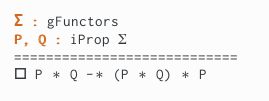
\includegraphics[scale=0.7]{sections/graphics/proofmode-0.png}
\end{center}
Ignoring $\Sigma$, which has to do with specifying which resource algebras are available, this is an ordinary Coq goal.
The assumptions are that $P$ and $Q$ are Iris propositions, and the goal is to prove the entailment.
Note that the $\vdash$ is replaced with $-\ast$, for reasons which are not important.
It is simply different notation for the same thing.

We then enter the proof mode at which point our goal looks as follows.
\begin{center}
  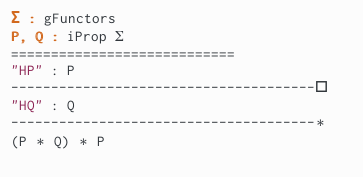
\includegraphics[scale=0.7]{sections/graphics/proofmode-1.png}
\end{center}
The Coq context, above the double line, stays the same, but the goal is different.
It consists of two contexts, and a conclusion.
The first context contains one assumption $P$, named \texttt{HP}.
Assumptions are named so that they can be referred to by tactics, analogously how assumptions are named in ordinary Coq proofs, except that for engineering reasons names of Iris assumptions need to be quoted as strings.
This is the context of \emph{persistent assumptions}.
Every assumption in this context implicitly has an $\persistently$ modality around it.

The second context also contains one assumption, $Q$, and the assumption has name \texttt{HQ}.
This is a context of arbitrary Iris assertions.

To prove the goal, if we were using the rules of the logic directly, we would duplicate the assumption $\persistently P$, and then use the separating conjunction introduction rule.
There is a tactic which corresponds to the separating conjunction introduction rule,\footnote{There are in fact two, \texttt{isSplitL}, and \texttt{iSplitR}.} and the tactic knows that persistent assertions can be duplicated.
Thus using this tactic we get the following two goals.
\begin{center}
  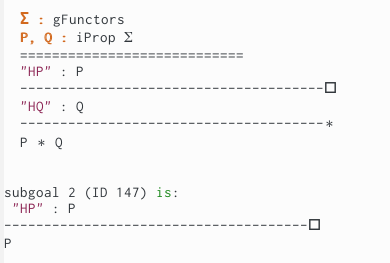
\includegraphics[scale=0.7]{sections/graphics/proofmode-2.png}
\end{center}
Notice how in the first goal we have assertions $P$ and $Q$ available, whereas in the second we only have $P$ available, since $Q$ is not persistent.

In the accompanying Coq example files we explain how to use the tactics and manipulate contexts to achieve this.

\paragraph*{Hoare triples in Iris Coq}
One point of difference of the Iris logic in Coq as opposed to the one presented in this paper is the definition of Hoare triples.
Recall that we defined Hoare triples as
\begin{align*}
  \hoare{P}{e}{\Phi} \eqdef \persistently\left(P \wand \wpre{e}{\Phi}\right).
\end{align*}
In Coq they are defined slightly differently, using the similar mode of use of weakest precondition specifications with an arbitrary postcondition.
To wit, they are defined as
\begin{align*}
  \hoare{P}{e}{\Phi}[\mask] \eqdef \persistently\left(\forall \Psi, P \wand \later(\forall v, \Phi(v) \wand \Psi(v)) \wand \wpre{e}[\mask]{\Psi}\right).
\end{align*}
If there was no later modality the two definitions would be rather trivially equivalent.
The reason for introducing the later modality is technical, and it is there purely for reasons of convenience.
\begin{exercise}
  Show that for expressions $e$ \emph{which are not values} the two definitions are logically equivalent.
\end{exercise}

Thus, the only place where they differ slightly is for values.
But since these triples are in practice never used for values, they are only used for top-level specifications, it does not matter.

%%% Local Variables:
%%% mode: latex
%%% TeX-master: "../main.tex"
%%% End:
